%!TEX root = Progetto.tex
\section{Progettazione Logica}
	\subsection{Tavola dei Volumi}
		\subsubsection{Tavola dei Volumi}
		\label{sec:volume_table}

			I volumi delle entità e delle relazioni sono stati stimati facendo riferimento ad un ciclo di vita della base di dati di circa 3 anni. In tale calcolo abbiamo considerato che alcune entità sono soggette ad una iniziale migrazione di dati (come ad esempio l'entità \emph{Fornitore} o \emph{Componente}).
		
			\begin{longtable}{| p{4cm} | p{4cm} | p{4cm} |}


				\hline
				\textbf{Concetto} & 
				\textbf{Tipo} & 
				\textbf{Volume} \\
				\hline
				
				\endfirsthead
				
				\hline
				\textbf{Concetto} & 
				\textbf{Tipo} & 
				\textbf{Volume} \\
				\hline
				\endhead
				
				Persona       & E & 495  \\ \hline
				Cliente       & E & 450  \\ \hline
				Privato       & E & 300  \\ \hline
				Azienda       & E & 150  \\ \hline
				Fornitore     & E & 42   \\ \hline
				Operatore     & E & 3    \\ \hline
				Autovettura   & E & 585  \\ \hline
				Preventivo    & E & 1500 \\ \hline
				Componente    & E & 472  \\ \hline
				Fornitura     & E & 1500 \\ \hline
				Ordine        & E & 300  \\ \hline
				Magazzino     & E & 189  \\ \hline
				Prestazione   & E & 1425 \\ \hline
				Turno         & E & 3000 \\ \hline
				Transazione   & E & 3747 \\ \hline
				Fattura       & E & 1425 \\ \hline
				Recapito      & E & 1077 \\ \hline
				Esecuzione    & R & 1425 \\ \hline
				Previsione    & R & 9000 \\ \hline
				Riferimento   & R & 1500 \\ \hline
				Formazione    & R & 1500 \\ \hline
				Composizione  & R & 472  \\ \hline
				Utilizzo      & R & 8550 \\ \hline
				Occupazione   & R & 2850 \\ \hline
				Presenza      & R & 3000 \\ \hline
				Possesso      & R & 585  \\ \hline
				Richiesta     & R & 1500 \\ \hline
				Acquisto      & R & 300  \\ \hline
				Rubrica       & R & 1077 \\ \hline
				Acconto       & R & 750  \\ \hline
				Registrazione & R & 1425 \\ \hline
				Pagamento     & R & 1425 \\ \hline
				Versamento    & R & 300  \\ \hline
				Salario       & R & 72   \\ \hline
				
			\end{longtable}
			
		\subsubsection{Tavola delle Operazioni}
		
			\begin{longtable}{| p{6.2cm} | p{6.2cm} |}

				\hline
				\textbf{Operazione} & 
				\textbf{Frequenza} \\
				\hline
				
				\endfirsthead
				
				\hline
				\textbf{Operazione} & 
				\textbf{Frequenza} \\
				\hline
				
				\endhead
				
				% Inserimenti
				\ref{op:new_cliente} & 3 volte a settimana \\ \hline
				\ref{op:new_privato} & 2 volte a settimana \\ \hline
				\ref{op:new_azienda} & 1 volta a settimana \\ \hline
				\ref{op:new_auto} & 3 volte a settimana \\ \hline
				\ref{op:new_fornitore} & 4 volte l'anno \\ \hline
				\ref{op:new_componente} & 2 volte al mese \\ \hline
				\ref{op:new_ordine} & 2 volte a settimana \\ \hline
				\ref{op:new_fornitura} & 10 volte a settimana \\ \hline
				\ref{op:new_preventivo} & 10 volte a settimana \\ \hline
				\ref{op:new_prestazione} & 10 volte a settimana \\ \hline
				\ref{op:new_fattura} & 10 volte a settimana \\ \hline
				\ref{op:new_operatore} & 1 volta all'anno \\ \hline
				\ref{op:new_recapito} & 80 volte ogni 3 mesi \\ \hline
				\ref{op:new_presenza} & 2 volte al giorno per ogni operatore \\ \hline
				\ref{op:new_transazione} & 18 volte a settimana \\ \hline

				% Assegnazioni
				\ref{op:ass_componente_preventivo} & 60 volte a settimana \\ \hline
				\ref{op:ass_componente_prestazione} & 60 volte a settimana \\ \hline
				\ref{op:ass_fornitura_ordine} & 10 volte a settimana \\ \hline
				\ref{op:ass_fornitura_magazzino} & 10 volte a settimana \\ \hline

				% Aggiornamenti
				\ref{op:edit_cliente} & 30 volte l'anno \\ \hline
				\ref{op:edit_fornitore} & 2 volte l'anno \\ \hline
				\ref{op:edit_operatore} & 1 volta l'anno \\ \hline
				\ref{op:edit_componente} & 5 volte al mese \\ \hline
				\ref{op:reg_ordine} & 2 volte a settimana \\ \hline

				% Consultazioni
				\ref{op:show_collaudo} & 1 volta a settimana \\ \hline
				\ref{op:show_revisione} & 1 volta a settimana \\ \hline
				\ref{op:show_fattura} & 10 volte a settimana \\ \hline
				\ref{op:show_transazioni} & 1 volta a settimana \\ \hline
				\ref{op:show_riparazioni} & 2 volte al giorno \\ \hline
				\ref{op:show_preventivi} & 2 volte al giorno \\ \hline
				\ref{op:check_componente} & 4 volte al giorno \\ \hline
				\ref{op:check_turni} & 1 volta al mese \\ \hline
				\ref{op:list_componenti} & 1 volta a settimana \\ \hline
				\ref{op:stats_componenti} & 2 volte al mese \\ \hline
				\ref{op:tobuy_componenti} & 1 volta a settimana \\ \hline
				\ref{op:show_recapiti_cliente} & 10 volte a settimana \\ \hline
				\ref{op:show_recapiti_fornitore} & 2 volte a settimana \\ \hline
				\ref{op:show_recapiti_operatore} & 1 volta a settimana \\ \hline
				\ref{op:list_fatture_pending} & 1 volta al giorno \\ \hline
				\ref{op:list_ordini_pending} & 1 volta a settimana \\ \hline
				\ref{op:todo_list} & 1 volta al giorno \\ \hline
				\ref{op:calc_stipendio_operatore} & 1 volta al mese per ogni operatore \\\hline
				\ref{op:stats_prevetivi_prestazioni} & 1 volta a settimana \\ \hline
				\ref{op:stats_costi} & 1 volta a settimana \\ \hline

			\end{longtable}
			
	\subsection{Ristrutturazione dello Schema Concettuale}

		\subsubsection{Analisi delle Derivazioni e della Ridondanza}

			Il modello elaborato nella precedente fase di sviluppo non rispondeva al criterio di minimalità. Gli attributi \emph{Imponibile} e \emph{Imposte} relativi all'entità \emph{Fattura} sono infatti attributi derivabili (Prendere in visione le Regole di Derivazione \ref{rd:imponibile} e \ref{rd:imposte}).

			Giunti ora all'ultima fase progettuale prima dell'effettiva implementazione della base di dati, ci occuperemo di valutare se eliminare o mantenere tale ridondanza, al fine da minimizzare i costi computazionali ed il numero di accessi. Inoltre valuteremo anche l'introduzione di ridondanze non presenti in precedenza, nel caso in cui tale introduzione apportasse sensibili miglioramenti alle prestazioni.

			Le stime degli accessi in lettura/scrittura verranno calcolate in riferimento ad un arco temporale pari ad un mese.

			Le operazioni legate agli attributi ridondanti \emph{Imponibile} ed \emph{Imposte} sono: \ref{op:new_fattura}, \ref{op:new_transazione}, \ref{op:show_fattura}).

			Abbiamo rintracciato altri dati derivabili utilizzati sistematicamente nelle nostre operazioni:

			\setenumerate[1]{label=\arabic*:}
			\begin{enumerate}

				\item \emph{Imponibile} relativo agli ordini effettuati presso i fornitori (\ref{op:new_ordine}\footnote{L'aggiunta di un nuovo ordine prevedere l'inserimento di nuove forniture. Nel calcolo degli accessi, calcoleremo anche questi ultimi}, \ref{op:new_transazione}));
			
				\item \emph{Quantità Presente} dei componenti in magazzino (\ref{op:reg_ordine}, \ref{op:check_componente}, \ref{op:list_componenti}, \ref{op:tobuy_componenti});
			
				\item \emph{Costo Componenti} relativo a \emph{Preventivo} (\ref{op:new_preventivo}, \ref{op:show_preventivi})
			
			\end{enumerate}

			\paragraph{\emph{Imponibile} in Fattura}

				L'\emph{Imponibile} di una fattura può essere ogni volta calcolato basandosi sui valori degli attributi:
				\setenumerate[1]{label=\arabic*)}
				\begin{enumerate}
					\item \emph{Quantità} ($q_i$) e \emph{Prezzo Unitario} ($p_i$) della relationship \emph{Utilizzo} che lega l'istanza della \emph{Prestazione} cui la fattura fa riferimento all'i-esima istanza di \emph{Fornitura}, in riferimento ai componenti utilizzati nella prestazione;
					\item \emph{Servizi Aggiuntivi} ($C_s$) e \emph{Manodopera} ($C_m$) relativi all'entità \emph{Prestazione};
					\item \emph{Sconto} ($S$), relativo all'entità \emph{Fattura}.
				\end{enumerate}

				$$ Imponibile = \left( C_s + C_m + \sum_{i=1}^n p_i q_i \right)\left(1 - \frac{S}{100}\right) $$

				Valutiamo la possibilità eliminare l'attributo ridondante \emph{Imponibile}.

				\subparagraph{Assenza di Ridondanza}
					Analizziamo il numero di accessi ipotizzando di non avere a disposizione l'attributo \emph{Imponibile} per l'entità \emph{Fattura}.

					\vspace{2ex}
					% Nuova fattura, no ridondanza
					\begin{tabular}{| p{3cm} | p{3cm} | p{3cm} | p{3cm} |}
						\hline
						\multicolumn{4}{|c|}{\textbf{\ref{op:new_fattura}}} \\ \hline
						\textbf{Concetto} & \textbf{Costrutto} & \textbf{Accessi} & \textbf{Tipo} \\ \hline
						Fattura & E & 1 & L \\
						Fattura & E & 1 & S \\
						\hline
					\end{tabular}

					% Nuova transazione, no ridondanza
					\begin{tabular}{| p{3cm} | p{3cm} | p{3cm} | p{3cm} |}
						\hline
						\multicolumn{4}{|c|}{\textbf{\ref{op:new_transazione}}} \\ \hline
						\textbf{Concetto} & \textbf{Costrutto} & \textbf{Accessi} & \textbf{Tipo} \\ \hline
						Fattura 		& E & 1 & L \\
						Prestazione 	& E & 1 & L \\
						Utilizzo 		& R & 6 & L \\
						Transazione 	& E & 1 & S \\
						\hline
					\end{tabular}

					% Dati per la stampa di fatture, no ridondanza
					\begin{tabular}{| p{3cm} | p{3cm} | p{3cm} | p{3cm} |}
						\hline
						\multicolumn{4}{|c|}{\textbf{\ref{op:show_fattura}}} \\ \hline
						\textbf{Concetto} & \textbf{Costrutto} & \textbf{Accessi} & \textbf{Tipo} \\ \hline
						Fattura 	& E & 1 & L \\
						Prestazione & E & 1 & L \\
						Utilizzo 	& R & 6 & L \\
						Preventivo 	& E & 1 & L \\
						Autovettura & E & 1 & L \\
						Cliente 	& E & 1 & L \\
						\hline
					\end{tabular}
					\vspace{2ex}

				\subparagraph{Presenza di Ridondanza} 
					Analizziamo il numero di accessi avendo a disposizione l'attributo \emph{Importo} relativo all'entità \emph{Fattura}.

					\vspace{2ex}
					% Nuova fattura, ridondanza
					\begin{tabular}{| p{3cm} | p{3cm} | p{3cm} | p{3cm} |}
						\hline
						\multicolumn{4}{|c|}{\textbf{\ref{op:new_fattura}}} \\ \hline
						\textbf{Concetto} & \textbf{Costrutto} & \textbf{Accessi} & \textbf{Tipo} \\ \hline
						Prestazione & E & 1 & L \\
						Utilizzo 	& R & 6 & L \\
						Fattura 	& E & 1 & L \\
						Fattura 	& E & 1 & S \\
						\hline
					\end{tabular}

					% Nuova transazione, ridondanza
					\begin{tabular}{| p{3cm} | p{3cm} | p{3cm} | p{3cm} |}
						\hline
						\multicolumn{4}{|c|}{\textbf{\ref{op:new_transazione}}} \\ \hline
						\textbf{Concetto} & \textbf{Costrutto} & \textbf{Accessi} & \textbf{Tipo} \\ \hline
						Fattura & E & 1 & L \\
						Transazione & E & 1 & S \\
						\hline
					\end{tabular}

					% Dati per la stampa di fatture, ridondanza
					\begin{tabular}{| p{3cm} | p{3cm} | p{3cm} | p{3cm} |}
						\hline
						\multicolumn{4}{|c|}{\textbf{\ref{op:show_fattura}}} \\ \hline
						\textbf{Concetto} & \textbf{Costrutto} & \textbf{Accessi} & \textbf{Tipo} \\ \hline
						Fattura & E & 1 & L \\
						Prestazione & E & 1 & L \\
						Autovettura & E & 1 & L \\
						Cliente & E & 1 & L \\
						\hline
					\end{tabular}
					\vspace{2ex}

				\subparagraph{Calcolo dei Costi Totali}
					Valutiamo la convenienza di lasciare o rimuovere l'attributi \emph{Imponibile} in \emph{Fattura}.

					\vspace{2ex}
					\begin{tabular}{| p{3cm} | p{3cm} | p{3cm} | p{3cm} |}
						\hline
						\textbf{Operazione} & \textbf{Costo} & \textbf{Frequenza} & \textbf{Totale} \\ \hline
						\ref{op:new_fattura} & 3 & $10 \cdot 4w = 40$ & 120 \\
						\ref{op:new_transazione} & 10 & $10 \cdot 4w = 40$ & 400 \\
						\ref{op:show_fattura} & 11 & $10 \cdot 4w = 40$ & 440 \\
						\hline
						\multicolumn{3}{|c|}{\textbf{Costo totale senza ridondanza}} & 960 \\
						\hline
					\end{tabular}

					\begin{tabular}{| p{3cm} | p{3cm} | p{3cm} | p{3cm} |}
						\hline
						\textbf{Operazione} & \textbf{Costo} & \textbf{Frequenza} & \textbf{Totale} \\ \hline
						\ref{op:new_fattura} & 10 & $10 \cdot 4w = 40$ & 400 \\
						\ref{op:new_transazione} & 3 & $10 \cdot 4w = 40$ & 120 \\
						\ref{op:show_fattura} & 4 & $10 \cdot 4w = 40$ & 160 \\
						\hline
						\multicolumn{3}{|c|}{\textbf{Costo totale con ridondanza}} & 680 \\
						\hline

					\end{tabular}
					\vspace{2ex}

					È conveniente lasciare l'attributo ridondante \emph{Imponibile} in \emph{Fattura}.

			\paragraph{\emph{Imposte} in Fattura}
				Le \emph{Imposte} in una fattura corrispondono all'ammontare dell'IVA. Attualmente l'IVA corrisponde al 22\% dell'\emph{Imponibile}. Ricordiamo che, anche in questo caso, le operazioni interessate sono: \ref{op:new_fattura}, \ref{op:new_transazione}, \ref{op:show_fattura}.

				Avendo a disposizione l'attributo \emph{Imponibile} nella stessa entità, il numero di accessi nel caso senza ridondanza risulta identico al caso con ridondanza. Possiamo fare a meno di tale dato ridondante.

				\begin{figure}[H]
					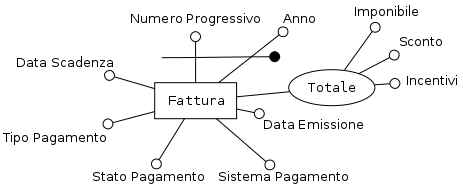
\includegraphics[width=9cm]{images/refactor/fattura.png}
					\centering
					\label{fig:fattura_refactor}
					\caption{Ristrutturazione di \emph{Fattura}}
				\end{figure}

			\paragraph{\emph{Imponibile} in Ordine}
				L'imponibile di un ordine corrisponde al costo delle forniture che lo compongono, su cui vanno calcolate le imposte. La somma di imponibile ed imposte di ordine, indica l'ammontare dell'effettiva transazione monetaria da parte dell'attività al fornitore presso cui è stato effettuato l'ordine.

				Valutiamo la possibilità di aggiungere l'attributo \emph{Imponibile} all'entità \emph{Ordine}.

				\subparagraph{Assenza di Ridondanza}
					Analizziamo il numero di accessi per le operazioni specificate senza introdurre dati ridondanti.

					\vspace{2ex}
					% Nuovo ordine, no ridondanza
					\begin{tabular}{| p{3cm} | p{3cm} | p{3cm} | p{3cm} |}
						\hline
						\multicolumn{4}{|c|}{\textbf{\ref{op:new_ordine}}} \\ \hline
						\textbf{Concetto} & \textbf{Costrutto} & \textbf{Accessi} & \textbf{Tipo} \\ \hline
						Fornitura 	& E & 5 & S \\
						Formazione 	& R & 5 & S \\
						Ordine 		& E & 1 & S \\
						\hline
					\end{tabular}

					% Nuova transazione, no ridondanza
					\begin{tabular}{| p{3cm} | p{3cm} | p{3cm} | p{3cm} |}
						\hline
						\multicolumn{4}{|c|}{\textbf{\ref{op:new_transazione}}} \\ \hline
						\textbf{Concetto} & \textbf{Costrutto} & \textbf{Accessi} & \textbf{Tipo} \\ \hline
						Ordine 		& E & 1 & L \\
						Formazione	& R & 5 & L \\
						Fornitura 	& E & 5 & L \\
						Transazione & E & 1 & S \\
						\hline
					\end{tabular}
					\vspace{2ex}

				\subparagraph{Presenza di Ridondanza}
					Analizziamo ora il numero di accessi introducendo l'attributo \emph{Imponibile} in \emph{Ordine}.

					\vspace{2ex}
					% Nuovo ordine, con ridondanza
					\begin{tabular}{| p{3cm} | p{3cm} | p{3cm} | p{3cm} |}
						\hline
						\multicolumn{4}{|c|}{\textbf{\ref{op:new_ordine}}} \\ \hline
						\textbf{Concetto} & \textbf{Costrutto} & \textbf{Accessi} & \textbf{Tipo} \\ \hline
						Fornitura 	& E & 5 & S \\
						Formazione 	& R & 5 & S \\
						Ordine 		& E & 1 & S \\
						\hline
					\end{tabular}

					% Nuova transazione, con ridondanza
					\begin{tabular}{| p{3cm} | p{3cm} | p{3cm} | p{3cm} |}
						\hline
						\multicolumn{4}{|c|}{\textbf{\ref{op:new_transazione}}} \\ \hline
						\textbf{Concetto} & \textbf{Costrutto} & \textbf{Accessi} & \textbf{Tipo} \\ \hline
						Ordine 		& E & 1 & L \\
						\hline
					\end{tabular}
					\vspace{2ex}

				\subparagraph{Calcolo dei Costi Totali}
					Valutiamo l'introduzione dell'attributo \emph{Imponibile} in \emph{Ordine}.

					\vspace{2ex}
					\begin{tabular}{| p{3cm} | p{3cm} | p{3cm} | p{3cm} |}
						\hline
						\textbf{Operazione} & \textbf{Costo} & \textbf{Frequenza} & \textbf{Totale} \\ \hline
						\ref{op:new_ordine} & 22 & $2 \cdot 4w = 8$ & 176 \\
						\ref{op:new_transazione} & 13 & $2 \cdot 4w = 8$ & 104 \\
						\hline
						\multicolumn{3}{|c|}{\textbf{Costo totale senza ridondanza}} & 280 \\
						\hline
					\end{tabular}

					\begin{tabular}{| p{3cm} | p{3cm} | p{3cm} | p{3cm} |}
						\hline
						\textbf{Operazione} & \textbf{Costo} & \textbf{Frequenza} & \textbf{Totale} \\ \hline
						\ref{op:new_ordine} & 22 & $2 \cdot 4w = 8$ & 176 \\
						\ref{op:new_transazione} & 1 & $2 \cdot 4w = 8$ & 8 \\
						\hline
						\multicolumn{3}{|c|}{\textbf{Costo totale con ridondanza}} & 184 \\
						\hline

					\end{tabular}
					\vspace{2ex}

					Conviene introdurre l'attributo \emph{Imponibile} nell'entità e \emph{Componente}.

					\begin{figure}[H]
						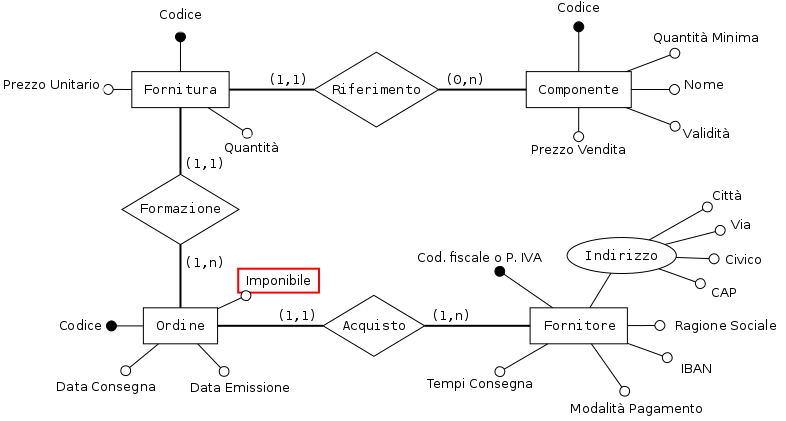
\includegraphics[width=12cm]{images/refactor/fornitore_ordine_fornitura_componente.png}
						\centering
						\label{fig:ordine_refactor}
						\caption{Ristrutturazione di \emph{Ordine}}
					\end{figure}

			\paragraph{\emph{Quantità} in Componente}
				Con \emph{Quantità}, riferito all'entità \emph{Componente}, si intende la quantità degli articoli per uno specifico componente disponibili in magazzino, a prescindere dalla fornitura d'appartenenza.
				Tale definizione fornisce la modalità con cui la quantità presente di un componente può essere calcolata fino a questo momento. Ci occuperemo di stabilire, ora, se possa essere vantaggioso introdurre tale dato derivabile come attributo dell'entità \emph{Componente}.

				\subparagraph{Assenza di Ridondanza}
					Analizziamo gli accessi necessari a svolgere le seguenti operazioni considerando il caso privo di dati ridondanti.

					\vspace{2ex}
					% Consegna ordine, senza ridondanza
					\begin{tabular}{| p{3cm} | p{3cm} | p{3cm} | p{3cm} |}
						\hline
						\multicolumn{4}{|c|}{\textbf{\ref{op:reg_ordine}}} \\ \hline
						\textbf{Concetto} & \textbf{Costrutto} & \textbf{Accessi} & \textbf{Tipo} \\ \hline
						Ordine 		& E & 1 & L \\
						Formazione	& R & 5 & L \\
						Fornitura 	& E & 5 & L \\
						Magazzino  	& E & 5 & S \\
						\hline
					\end{tabular}

					% Controlla componente, no ridondanza
					\begin{tabular}{| p{3cm} | p{3cm} | p{3cm} | p{3cm} |}
						\hline
						\multicolumn{4}{|c|}{\textbf{\ref{op:check_componente}}} \\ \hline
						\textbf{Concetto} & \textbf{Costrutto} & \textbf{Accessi} & \textbf{Tipo} \\ \hline
						Componente 	& E & 1 & L \\
						Magazzino 	& E & 1\footnotemark & L \\
						\hline
					\end{tabular}

					\footnotetext{Valore medio. Per i componenti non presenti in magazzino non ci sarà alcun accesso, per quelli presenti ci saranno tanti accessi quante sono le forniture non ancora esaurite.}

					% Lista componenti presenti, no ridondanza
					\begin{tabular}{| p{3cm} | p{3cm} | p{3cm} | p{3cm} |}
						\hline
						\multicolumn{4}{|c|}{\textbf{\ref{op:list_componenti}}} \\ \hline
						\textbf{Concetto} & \textbf{Costrutto} & \textbf{Accessi} & \textbf{Tipo} \\ \hline
						Magazzino 	& E & $1 \cdot 189=189$ \footnotemark & L \\
						Componente 	& E & $1 \cdot 189=189$ \footnotemark & L \\
						\hline
					\end{tabular}
					\footnotetext{Quantità derivante dalla Tavolta dei Volumi \ref{sec:volume_table}. Sebbene la Tavola dei Volumi sia riferita ad un arco temporale di 3 anni, il volume dell'entità \emph{Magazzino} rimane pressoché costante nel tempo.}
					\footnotetext{Stima massimale. Ad ogni istanza di \emph{Componente} possono corrispondere più istanze di \emph{Magazzino}.}

					% Lista componenti da comprare, no ridondanza
					\begin{tabular}{| p{3cm} | p{3cm} | p{3cm} | p{3cm} |}
						\hline
						\multicolumn{4}{|c|}{\textbf{\ref{op:tobuy_componenti}}} \\ \hline
						\textbf{Concetto} & \textbf{Costrutto} & \textbf{Accessi} & \textbf{Tipo} \\ \hline
						Magazzino 	& E & $1 \cdot 189=189$ & L \\
						Componente 	& E & $1 \cdot 189=189$ & L \\
						\hline
					\end{tabular}
					\vspace{2ex}

				\subparagraph{Presenza di Ridondanza}
					Analizziamo nuovamente il numero di accessi considerando l'attributo ridondante \emph{Quantità}.

					\vspace{2ex}
					% Consegna ordine, con ridondanza
					\begin{tabular}{| p{3cm} | p{3cm} | p{3cm} | p{3cm} |}
						\hline
						\multicolumn{4}{|c|}{\textbf{\ref{op:reg_ordine}}} \\ \hline
						\textbf{Concetto} & \textbf{Costrutto} & \textbf{Accessi} & \textbf{Tipo} \\ \hline
						Ordine 		& E & 1 & L \\
						Formazione	& R & 5 & L \\
						Fornitura 	& E & 5 & L \\
						Magazzino  	& E & 5 & S \\
						Componente 	& E & 1 & L \\
						Componente 	& E & 1 & S \\
						\hline
					\end{tabular}

					% Controlla componente, con ridondanza
					\begin{tabular}{| p{3cm} | p{3cm} | p{3cm} | p{3cm} |}
						\hline
						\multicolumn{4}{|c|}{\textbf{\ref{op:check_componente}}} \\ \hline
						\textbf{Concetto} & \textbf{Costrutto} & \textbf{Accessi} & \textbf{Tipo} \\ \hline
						Componente 	& E & 1 & L \\
						\hline
					\end{tabular}

					% Lista componenti presenti, con ridondanza
					\begin{tabular}{| p{3cm} | p{3cm} | p{3cm} | p{3cm} |}
						\hline
						\multicolumn{4}{|c|}{\textbf{\ref{op:list_componenti}}} \\ \hline
						\textbf{Concetto} & \textbf{Costrutto} & \textbf{Accessi} & \textbf{Tipo} \\ \hline
						Componente 	& E & $1 \cdot 472 = 472$ \footnotemark & L \\
						\hline
					\end{tabular}
					\footnotetext{Dalla Tavola dei Volumi \ref{sec:volume_table}}

					% Lista componenti da comprare, con ridondanza
					\begin{tabular}{| p{3cm} | p{3cm} | p{3cm} | p{3cm} |}
						\hline
						\multicolumn{4}{|c|}{\textbf{\ref{op:tobuy_componenti}}} \\ \hline
						\textbf{Concetto} & \textbf{Costrutto} & \textbf{Accessi} & \textbf{Tipo} \\ \hline
						Componente 	& E & $1 \cdot 472 = 472$ & L \\
						\hline
					\end{tabular}
					\vspace{2ex}

				\subparagraph{Calcolo dei Costi Totali}
					Valutiamo l'introduzione dell'attributo \emph{Quantità} in \emph{Componente}.

					\vspace{2ex}
					\begin{tabular}{| p{3cm} | p{3cm} | p{3cm} | p{3cm} |}
						\hline
						\textbf{Operazione} & \textbf{Costo} & \textbf{Frequenza} & \textbf{Totale} \\ \hline
						\ref{op:reg_ordine}			& 21	& $2 \cdot 4w = 8$		& 168 	\\
						\ref{op:check_componente}	& 2 	& $4 \cdot 24d = 96$	& 192	\\
						\ref{op:list_componenti}	& 378	& $1 \cdot 4w = 4$		& 1512	\\ 
						\ref{op:tobuy_componenti}	& 378	& $1 \cdot 4w = 4$		& 1512	\\
						\hline
						\multicolumn{3}{|c|}{\textbf{Costo totale senza ridondanza}} & 3384 \\
						\hline
					\end{tabular}

					\begin{tabular}{| p{3cm} | p{3cm} | p{3cm} | p{3cm} |}
						\hline
						\textbf{Operazione} & \textbf{Costo} & \textbf{Frequenza} & \textbf{Totale} \\ \hline
						\ref{op:reg_ordine}			& 24	& $2 \cdot 4w = 8$		& 192 	\\
						\ref{op:check_componente}	& 1 	& $4 \cdot 24d = 96$	& 96	\\
						\ref{op:list_componenti}	& 472	& $1 \cdot 4w = 4$		& 1888	\\ 
						\ref{op:tobuy_componenti}	& 472	& $1 \cdot 4w = 4$		& 1888	\\
						\hline
						\multicolumn{3}{|c|}{\textbf{Costo totale con ridondanza}} & 4064 \\
						\hline
					\end{tabular}
					\vspace{2ex}

					L'introduzione dell'attributo \emph{Quantità} in \emph{Componente} aumenterebbe il numero di accessi necessari ad eseguire le operazioni necessarie. Non è necessaria alcuna ristrutturazione.

			\paragraph{\emph{Costo Componenti} in Preventivo}
				L'entità \emph{Componente} è soggetta ad operazioni simili a quelle cui sono soggette le entità \emph{Fattura} ed \emph{Ordine}, quindi è ragionevole valutare l'evenienza di aggiungere il dato derivabile \emph{Costo Componenti}.

				\subparagraph{Assenza di Ridondanza}
					Analizziamo il numero degli accessi necessari per effettuare le operazioni allo stato attuale del modello.

					\vspace{2ex}
					% Nuovo preventivo, no ridondanza
					\begin{tabular}{| p{3cm} | p{3cm} | p{3cm} | p{3cm} |}
						\hline
						\multicolumn{4}{|c|}{\textbf{\ref{op:new_preventivo}}} \\ \hline
						\textbf{Concetto} & \textbf{Costrutto} & \textbf{Accessi} & \textbf{Tipo} \\ \hline
						Preventivo 		& E & 1 & S \\
						Componente 		& E & 6 & L \\
						Previsione		& R & 6 & S \\
						\hline
					\end{tabular}

					% Show preventivo, no ridondanza
					\begin{tabular}{| p{3cm} | p{3cm} | p{3cm} | p{3cm} |}
						\hline
						\multicolumn{4}{|c|}{\textbf{\ref{op:show_preventivi}}} \\ \hline
						\textbf{Concetto} & \textbf{Costrutto} & \textbf{Accessi} & \textbf{Tipo} \\ \hline
						Preventivo 		& E & 1 & L \\
						Previsione		& R & 6 & L \\
						\hline
					\end{tabular}
					\vspace{2ex}

				\subparagraph{Presenza di Ridondanza}
					Vediamo ora il numero di accessi introducendo l'attributo \emph{Costo Componenti} in \emph{Preventivo}.

					\vspace{2ex}
					% Nuovo preventivo, con ridondanza
					\begin{tabular}{| p{3cm} | p{3cm} | p{3cm} | p{3cm} |}
						\hline
						\multicolumn{4}{|c|}{\textbf{\ref{op:new_preventivo}}} \\ \hline
						\textbf{Concetto} & \textbf{Costrutto} & \textbf{Accessi} & \textbf{Tipo} \\ \hline
						Componente 		& E & 6 & L \\
						Preventivo 		& E & 1 & S \\
						Previsione		& R & 6 & S \\
						\hline
					\end{tabular}

					% Show preventivo, con ridondanza
					\begin{tabular}{| p{3cm} | p{3cm} | p{3cm} | p{3cm} |}
						\hline
						\multicolumn{4}{|c|}{\textbf{\ref{op:show_preventivi}}} \\ \hline
						\textbf{Concetto} & \textbf{Costrutto} & \textbf{Accessi} & \textbf{Tipo} \\ \hline
						Preventivo 		& E & 1 & L \\
						\hline
					\end{tabular}
					\vspace{2ex}

				\subparagraph{Calcolo dei Costi Totali}

					Calcoliamo i costi totali nei due casi.

					\vspace{2ex}
					\begin{tabular}{| p{3cm} | p{3cm} | p{3cm} | p{3cm} |}
						\hline
						\textbf{Operazione} & \textbf{Costo} & \textbf{Frequenza} & \textbf{Totale} \\ \hline
						\ref{op:new_preventivo}		& 20 	& $10 \cdot 4w = 40$	& 800	\\
						\ref{op:show_preventivi} 	& 7 	& $2 \cdot 24d = 48$	& 336	\\
						\hline
						\multicolumn{3}{|c|}{\textbf{Costo totale senza ridondanza}} & 1136 \\
						\hline
					\end{tabular}

					\begin{tabular}{| p{3cm} | p{3cm} | p{3cm} | p{3cm} |}
						\hline
						\textbf{Operazione} & \textbf{Costo} & \textbf{Frequenza} & \textbf{Totale} \\ \hline
						\ref{op:new_preventivo}		& 20 	& $10 \cdot 4w = 40$	& 800	\\
						\ref{op:show_preventivi} 	& 1 	& $2 \cdot 24d = 48$	& 48	\\
						\hline
						\multicolumn{3}{|c|}{\textbf{Costo totale con ridondanza}} & 848 \\
						\hline
					\end{tabular}
					\vspace{2ex}

					È conveniente inserire l'attributo ridondante \emph{Costo Componenti} all'entità \emph{Preventivo}, alla luce dei risultati ottenuti.

					\begin{figure}[H]
						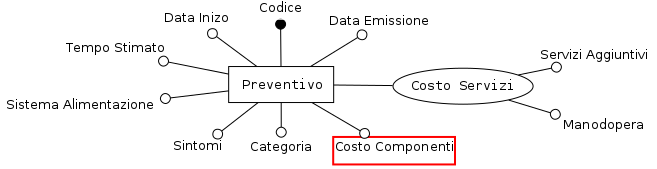
\includegraphics[width=11cm]{images/refactor/preventivo.png}
						\centering
						\label{fig:preventivo_refactor}
						\caption{Ristrutturazione di \emph{Preventivo}}
					\end{figure}

		\subsubsection{Eliminazione delle Generalizzazioni}

			Il modello concettuale, su cui ci stiamo basando in questa fase progettuale, non è ancora adeguato ad essere tradotto in un modello logico. Le generalizzazioni, che con questo passo andremo ad eliminare, sono dei costrutti del modello concettuale che permettono di modellare agevolmente la realtà d'interesse, ma che purtroppo non sono disponibili nel modello relazionale.

			Nel nostro modello concettuale sono presenti due generalizzazioni, quella che coinvolge le entità \emph{Cliente}, \emph{Fornitore} ed \emph{Operatore}, e quella che coinvolge le entità \emph{Privato} ed \emph{Azienda}.

			\begin{description}
				\item [Cliente] 
					Riguardo l'entità \emph{Cliente} abbiamo scelto di accorpare in essa le entità figlie. La motivazione principale sta nel fatto che, effettivamente, le entità figlie non sono direttamente in relazione con nessun'altra parte del modello che fin'ora abbiamo sviluppato.

				\item [Persona]
					Per quanto riguarda le invece le entità figlie di \emph{Persona}, l'accorpamento delle figlie nell'entità padre non è una strada percorribile, sia dal punto di vista tecnico (tale accorpamento genererebbe una tabella troppo corposa, con parecchi valori \emph{NULL}), sia dal punto di vista concettuale (tali entità modellano persone che hanno dei ruoli totalmente diversi tra loro all'interno dell'azienda).

					La scelta che ci sembra più adeguata per questa generalizzazione è quella di accorpare l'entità padre nelle entità figlie, rendendo isolate ed indipendenti tra loro le entità \emph{Cliente}, \emph{Fornitore} e \emph{Operatore}.
			\end{description}

			\begin{figure}[H]
				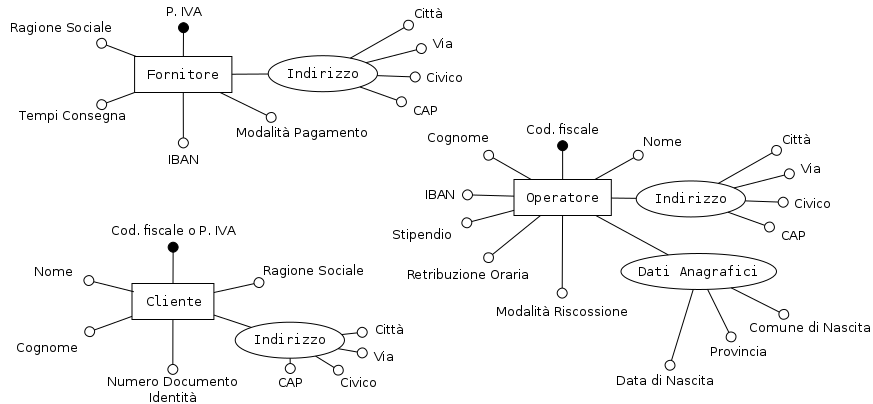
\includegraphics[width=13cm]{images/refactor/persona.png}
				\centering
				\label{fig:persona_refactor}
				\caption{Eliminazione delle generalizzazioni}
			\end{figure}
			
		\subsubsection{Partizionamento e Accorpamento di Concetti}

			\paragraph{Partizionamento di Concetti}
				L'eliminazione dell'entità padre \emph{Persona} induce un partizionamento della relationship \emph{Rubrica} con la quale veniva associata all'entità \emph{Recapito}.

				Il partizionamento più naturale per tale relationship ricalca il concetto della separazione delle entità \emph{Cliente}, \emph{Fornitore} e \emph{Operatore} effettuata nel precedente passo.

				Tale relationship sarà sostituita da tre relationship distinte (figura \ref{fig:rubrica_refactor}): \emph{Rubrica Cliente}, \emph{Rubrica Fornitore} e \emph{Rubrica Operatore}.

				Da notare sono le partecipazioni delle entità alle relationship. Nella fase progettuale precedente era stato necessario permettere che più istanze di \emph{Recapito} potessero partecipare alla relationship \emph{Rubrica}. Con l'eliminazione delle gerarchie ed il partizionamento della relationship, possiamo vincolare le partecipazioni con più precisione: permetteremo solamente alla relationship \emph{Rubrica Cliente} di accettare più istanze di \emph{Recapito} per la stessa istanza di \emph{Cliente}.

				\begin{sidewaysfigure}
					\centering
					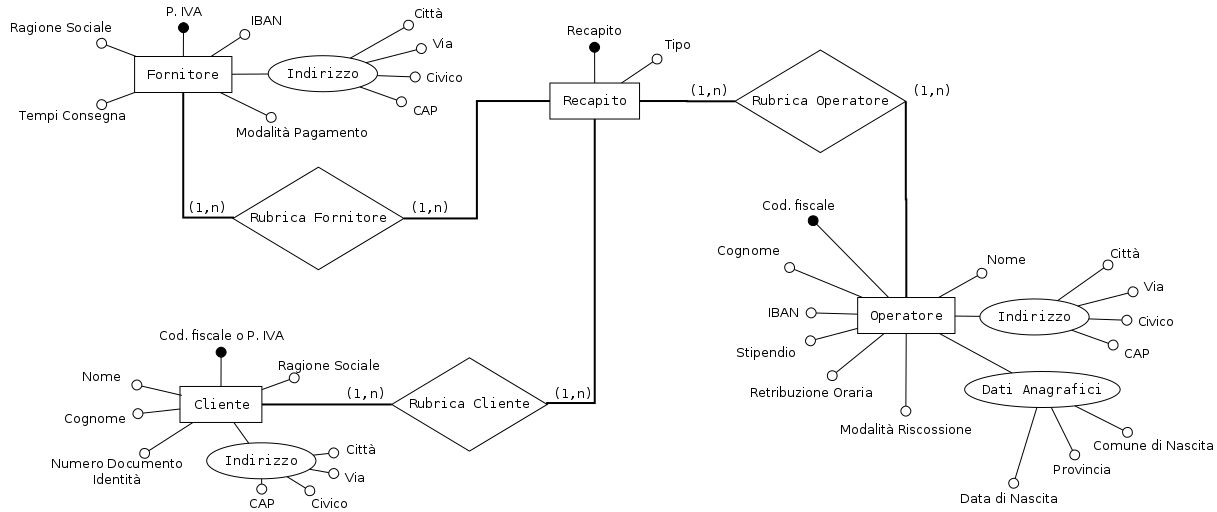
\includegraphics[width=22cm]{images/refactor/persona-recapito.png}
					\caption{Partizionamento di Rubrica}
					\label{fig:rubrica_refactor}
				\end{sidewaysfigure}

	\subsection{Scelta degli Identificatori Principali}

		Per quanto possibile, abbiamo scelto degli identificatori primari che fossero il più possibile significativi per ognuna delle entità. Purtroppo non abbiamo trovato degli identificativi, per così dire, \emph{naturali} tra gli attributi delle entità quali \emph{Componente}, \emph{Preventivo}, \emph{Fornitura} ed \emph{Ordine}, dovendo introdurre dei codici identificativi interni.

		Per alcune entità, come \emph{Fattura} e \emph{Magazzino}, mantenuto le superchiavi evitando di aggiungere altri attributi \emph{Codice}, con il fine di mantenere le rappresentazioni dei concetti che modellano, fedeli alla realtà.

		Per quanto riguarda invece l'entità \emph{Turno}, sembrava effettivamente superfluo e poco intuitivo insierire un attributo che fungesse da identificatore primario.

		In figura \ref{fig:schema_refactor} troviamo l'intero modello ER alla fine della sua ristrutturazione.
		
		\vspace{2ex}
		\begin{longtable}{| p{3cm} | p{9.4cm} |}
			\hline
			\textbf{Nome Entità} & \textbf{Identificatore} \\
			\hline
			\endfirsthead

			\hline
			\textbf{Nome Entità} & \textbf{Identificatore} \\
			\hline
			\endhead

			Cliente 		& Codice Fiscale o P.IVA 	\\ \hline
			Fornitore 		& Partita IVA 				\\ \hline
			Operatore 		& Codice Fiscale 			\\ \hline
			Autovettura  	& Targa						\\ \hline
			Preventivo 		& Codice					\\ \hline
			Componente 		& Codice					\\ \hline
			Fornitura 		& Codice					\\ \hline
			Ordine 			& Codice					\\ \hline
			Magazzino  		& Codice Componente, Codice (di \emph{Fornitura}			\\ \hline
			Prestazione 	& Codice (di \emph{Preventivo})								\\ \hline
			Turno			& Ora Inizio, Data, Codice Fiscale (di \emph{Operatore})	\\ \hline
			Transazione 	& Codice					\\ \hline
			Fattura         & Numero Progressivo, Anno 	\\ \hline
			Recapito 		& Recapito 					\\

			\hline			
		\end{longtable}
		\vspace{2ex}

		\begin{sidewaysfigure}
			\centering
			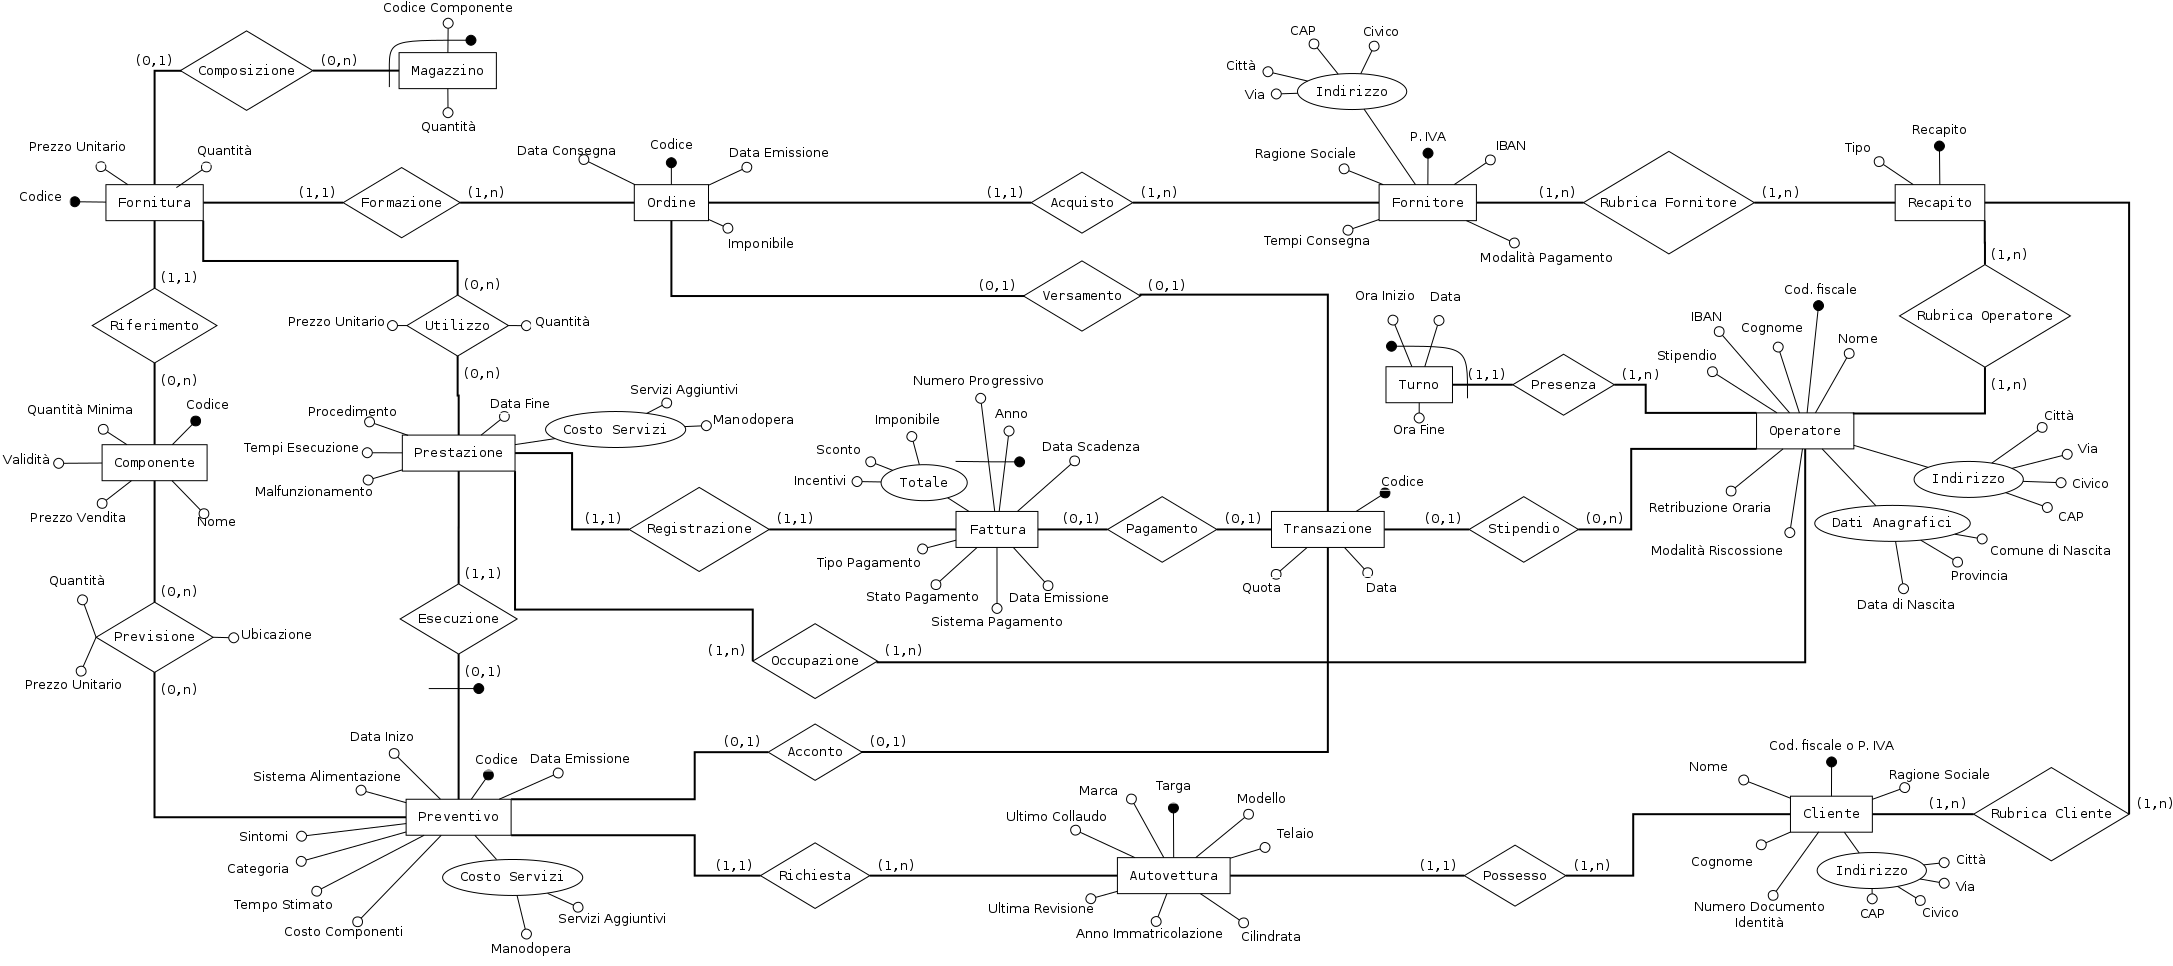
\includegraphics[width=22cm]{images/refactor/schema.png}
			\caption{Diagramma Entity-Relationship Ristrutturato}
			\label{fig:schema_refactor}
		\end{sidewaysfigure}

	\subsection{Normalizzazione}

		Dallo schema concettuale ristrutturato, notiamo che tutte le relationship sono già in BCNF, in quanto tutte binarie.

		\vspace{2ex}
		\begin{longtable}{| p{2.5cm} | p{12cm} |}
			\hline
			\textbf{Nome Entità} & \textbf{Identificatore} \\
			\hline
			\endfirsthead

			\hline
			\textbf{Nome Entità} & \textbf{Identificatore} \\
			\hline
			\endhead

			Cliente 		& Non esistono dipendenze non banali tra gli attributi 	\\ \hline
			Fornitore 		& Non esistono dipendenze non banali tra gli attributi	\\ \hline
			Operatore 		& Non esistono dipendenze non banali tra gli attributi	\\ \hline
			Autovettura		& È in terza forma normale	\\
							& $Telaio \rightarrow Targa, Marca, Modello, Cilindrata, Anno Immatricolazione$ \\
							& Telaio è superchiave, Targa è la chiave di Autovettura \\ \hline
			Preventivo 		& Non esistono dipendenze non banali tra gli attributi	\\ \hline
			Componente		& È in terza forma normale	\\
							& $Nome \rightarrow Codice, Prezzo Vendita, Validit\acute{a}, Quantit\acute{a} Minima$ \\
							& Nome è superchiave, Codice è la chiave di Componente  \\ \hline
			Fornitura 		& Non esistono dipendenze non banali tra gli attributi	\\ \hline
			Ordine 			& Non esistono dipendenze non banali tra gli attributi	\\ \hline
			Magazzino  		& Non esistono dipendenze non banali tra gli attributi	\\ \hline
			Prestazione 	& Non esistono dipendenze non banali tra gli attributi	\\ \hline
			Turno			& Non esistono dipendenze non banali tra gli attributi	\\ \hline
			Transazione 	& Non esistono dipendenze non banali tra gli attributi	\\ \hline
			Fattura         & Non esistono dipendenze non banali tra gli attributi	\\ \hline
			Recapito 		& Non esistono dipendenze non banali tra gli attributi	\\

			\hline			
		\end{longtable}
		\vspace{2ex}
		
	\subsection{Traduzione verso il Modello Relazionale}

	\vspace{2ex}
		\begin{longtable}{| p{3cm} | p{11.5cm} |}
			\hline
			\textbf{Entità/Relazione} & \textbf{Traduzione} \\
			\hline
			\endfirsthead

			\hline
			\textbf{Entità/Relazione} & \textbf{Traduzione} \\
			\hline
			\endhead

			Cliente & 
				Cliente(\underline{CF\_PIVA}, Nome, Cognome, RagioneSociale, Citta, Via, Civico, CAP, NDocID) \\
				\hline
			Fornitore &
				Fornitore(\underline{PIVA}, RagioneSociale, TempiConsegna, ModPagamento, IBAN, Citta, Via, Civico, CAP) \\
				\hline
			Operatore &
				Operatore(\underline{CF}, Nome, Cognome, Citta, Via, Civico, CAP, DataNasc, ComuneNasc, ProvinciaNasc, Stipendio, RetribuzioneH, ModRiscossione, IBAN) \\
				\hline
			Transazione &
				Transazione(\underline{Codice}, Quota, Data) \\
				\hline
			Autovettura &
				Autovettura(\underline{Targa}, Telaio, Marca, Modello, Cilindrata, AnnoImmatricolazione, UltimoCollaudo, UltimaRevisione, Cliente) \\
				\hline
			Preventivo &
				Preventivo(\underline{Codice}, DataEmissione, DataInizio, Categoria, Sintomi, SisAlimentazione, TempoStimato, CostoComponenti, Manodopera, ServAggiuntivi, Autovettura, Acconto) \\
				\hline
			Componente & 
				Componente(\underline{Codice}, Nome, QuantitaMin, Validita, PrezzoVendita) \\
				\hline
			Previsione &
				Previsione(\underline{Componente}, \underline{Preventivo}, Ubicazione, Quantita, PrezzoUnitario) \\
				\hline
			Prestazione &
				Prestazione(\underline{Preventivo}, TempiEsecuzione, Procedimento, DataFine, Malfunzionamento, ServAggiuntivi, Manodopera) \\
				\hline
			Occupazione &
				Occupazione(\underline{Prestazione}, \underline{Operatore}) \\
				\hline
			Ordine &
				Ordine(\underline{Codice}, DataEmissione, DataConsegna, Imponibile, Fornitore, Versamento) \\
				\hline
			Fornitura & 
				Fornitura(\underline{Codice}, Componente, Quantita, PrezzoUnitario, Ordine) \\
				\hline
			Utilizzo &
				Utilizzo(\underline{Prestazione}, \underline{Fornitura}, PrezzoUnitario, Quantita) \\
				\hline
			Magazzino &
				Magazzino(\underline{Componente}, \underline{Fornitura}, Quantita) \\
				\hline
			Fattura &
				Fattura(\underline{Numero}, \underline{Anno}, Prestazione, Imponibile, Sconto, Incentivi, DataEmissione, DataScadenza, TipoPag, StatoPag, SisPag, Transazione) \\
				\hline
			Turno & 
				Turno(\underline{Operatore}, \underline{Data}, \underline{OraInizio}, OraFine) \\
				\hline
			Stipendio &
				Stipendio(\underline{Transazione}, Operatore) \\
				\hline
			Recapito &
				Recapito(\underline{Recapito}, Tipo) \\
				\hline
			RubricaCliente &
				RubricaCliente(\underline{Recapito}, \underline{Cliente}) \\
				\hline
			RubricaFornitore &
				RubricaFornitore(\underline{Recapito}, \underline{Fornitore}) \\
				\hline
			RubricaOperatore &
				RubricaOperatore(\underline{Recapito}, \underline{Operatore}) \\
				\hline

		\end{longtable}
	\vspace{2ex}

	\vspace{2ex}
		\begin{longtable}{| p{8cm} | p{6.5cm} |}
			\hline
			\textbf{Traduzioni} & \textbf{Vincoli di Riferimento} \\
			\hline
			\endfirsthead

			\hline
			\textbf{Traduzioni} & \textbf{Vincoli di Riferimento} \\
			\hline
			\endhead

			Cliente(\underline{CF\_PIVA}, Nome, Cognome, RagioneSociale, Citta, Via, Civico, CAP, NDocID) &
			* \\ \hline
			Fornitore(\underline{PIVA}, RagioneSociale, TempiConsegna, ModPagamento, IBAN, Citta, Via, Civico, CAP) &
			* \\ \hline
			Operatore(\underline{CF}, Nome, Cognome, Citta, Via, Civico, CAP, DataNasc, ComuneNasc, ProvinciaNasc, Stipendio, RetribuzioneH, ModRiscossione, IBAN) &
			* \\ \hline
			Transazione(\underline{Codice}, Quota, Data) &
			* \\ \hline
			Autovettura(\underline{Targa}, Telaio, Marca, Modello, Cilindrata, AnnoImmatricolazione, UltimoCollaudo, UltimaRevisione, Cliente) &
			$Cliente \rightarrow Cliente.CF\_PIVA$ \\ 
			\hline
			Preventivo(\underline{Codice}, DataEmissione, DataInizio, Categoria, Sintomi, SisAlimentazione, TempoStimato, CostoComponenti, Manodopera, ServAggiuntivi, Autovettura, Acconto) &
			$Autovettura \rightarrow Autovettura.Targa$ \\
			& $Acconto \rightarrow Transazione.Codice$ \\
			\hline
			Componente(\underline{Codice}, Nome, QuantitaMin, Validita, PrezzoVendita) &
			* \\ \hline
			Previsione(\underline{Componente}, \underline{Preventivo}, Ubicazione, Quantita, PrezzoUnitario) &
			$Componente \rightarrow Componente.Codice$ \\
			& $Preventivo \rightarrow Preventivo.Codice$ \\
			\hline
			Prestazione(\underline{Preventivo}, TempiEsecuzione, Procedimento, DataFine, Malfunzionamento, ServAggiuntivi, Manodopera) &
			$Preventivo \rightarrow Preventivo.Codice$ \\
			\hline
			Occupazione(\underline{Prestazione}, \underline{Operatore}) &
			$Prestazione \rightarrow Prestazione.Preventivo$ \\
			& $Operatore \rightarrow Operatore.CF$ \\
			\hline
			Ordine(\underline{Codice}, DataEmissione, DataConsegna, Imponibile, Fornitore, Versamento) &
			$Versamento \rightarrow Transazione.Codice$ \\
			\hline
			Fornitura(\underline{Codice}, Componente, Quantita, PrezzoUnitario, Ordine) &
			$Componente \rightarrow Componente.Codice$ \\
			& $Ordine \rightarrow Ordine.Codice$ \\
			\hline
			Utilizzo(\underline{Prestazione}, \underline{Fornitura}, PrezzoUnitario, Quantita) &
			$Prestazione \rightarrow Prestazione.Preventivo$ \\
			& $Fornitura \rightarrow Fornitura.Codice$ \\
			\hline
			Magazzino(\underline{Componente}, \underline{Fornitura}, Quantita) &
			$Componente \rightarrow Componente.Codice$ \\
			& $Fornitura \rightarrow Fornitura.Codice$ \\
			\hline
			Fattura(\underline{Numero}, \underline{Anno}, Prestazione, Imponibile, Sconto, Incentivi, DataEmissione, DataScadenza, TipoPag, StatoPag, SisPag, Transazione) &
			$Prestazione \rightarrow Prestazione.Preventivo$ \\
			& $Transazione \rightarrow Transazione.Codice$ \\
			\hline
			Turno(\underline{Operatore}, \underline{Data}, \underline{OraInizio}, OraFine) &
			$Operatore \rightarrow Operatore.CF$ \\
			\hline
			Stipendio(\underline{Transazione}, Operatore) &
			$Transazione \rightarrow Transazione.Codice$ \\
			& $Operatore \rightarrow Operatore.CF$ \\
			\hline
			Recapito(\underline{Recapito}, Tipo) &
			* \\ \hline
			RubricaCliente(\underline{Recapito}, \underline{Cliente}) &
			$Recapito \rightarrow Recapito.Recapito$ \\
			& $Cliente \rightarrow Cliente.CF\_PIVA$ \\
			\hline
			RubricaFornitore(\underline{Recapito}, \underline{Fornitore}) &
			$Recapito \rightarrow Recapito.Recapito$ \\
			& $Fornitore \rightarrow Fornitore.PIVA$ \\
			\hline
			RubricaOperatore(\underline{Recapito}, \underline{Operatore}) &
			$Recapito \rightarrow Recapito.Recapito$ \\
			& $Operatore \rightarrow Operatore.CF$ \\
			\hline

		\end{longtable}
	\vspace{2ex}